\section{MEWE: Multi-variant Execution for WebAssembly}
\label{section:mewe}

\renewcommand{\tool}{MEWE\xspace}
\newcommand{\repourl}{TODO}
% Overview
This section describes MEWE \cite{MEWE}. 
\tool synthesizes diversified function variants by using CROW.
It then provides execution-path randomization in a Multivariant Execution (MVE).
The tool generates application-level multivariant binaries without changing the operating system or \wasm runtime.
MEWE creates an MVE by intermixing functions for which CROW generates variants, as step \step{2} in \autoref{diagrams:generic} shows.
CROW generates each one of these variants with fine-grained diversification at the instruction level, applying the majority of the strategies discussed in \autoref{sota:sota} and \emph{constant inferring}. \tool adds a new mutation strategy. It inlines function variants when appropriate, resulting in call stack diversification at runtime.

In \autoref{workflow} we zoom MEWE from the blue highlighted square in \autoref{diagrams:generic}. MEWE takes the LLVM IR variants generated by CROW's diversifier. It then merges LLVM IR variants into a Wasm multivariant.
In the figure, we highlight the two components of MEWE, \emph{Multivariant Generation} and the \emph{Mixer}.
In the \emph{Multivariant Generation} process, 
MEWE merges the LLVM IR variants created by CROW and creates an LLVM multivariant binary.
The merging of the variants intermixes the calling of function variants, making possible the execution path randomization.

\emph{The Mixer} augments the LLVM multivariant binary with a random generator. The random generator is needed to perform the execution-path randomization.
Also, \emph{The Mixer} fixes the entrypoint in the multivariant binary.
Finally, MEWE generates a standalone multivariant \wasm binary using the same custom Wasm LLVM backend from CROW.
Once generated, the generated multivariant \wasm binary can be deployed to any \wasm engine. 

\begin{figure*}
  \centering
  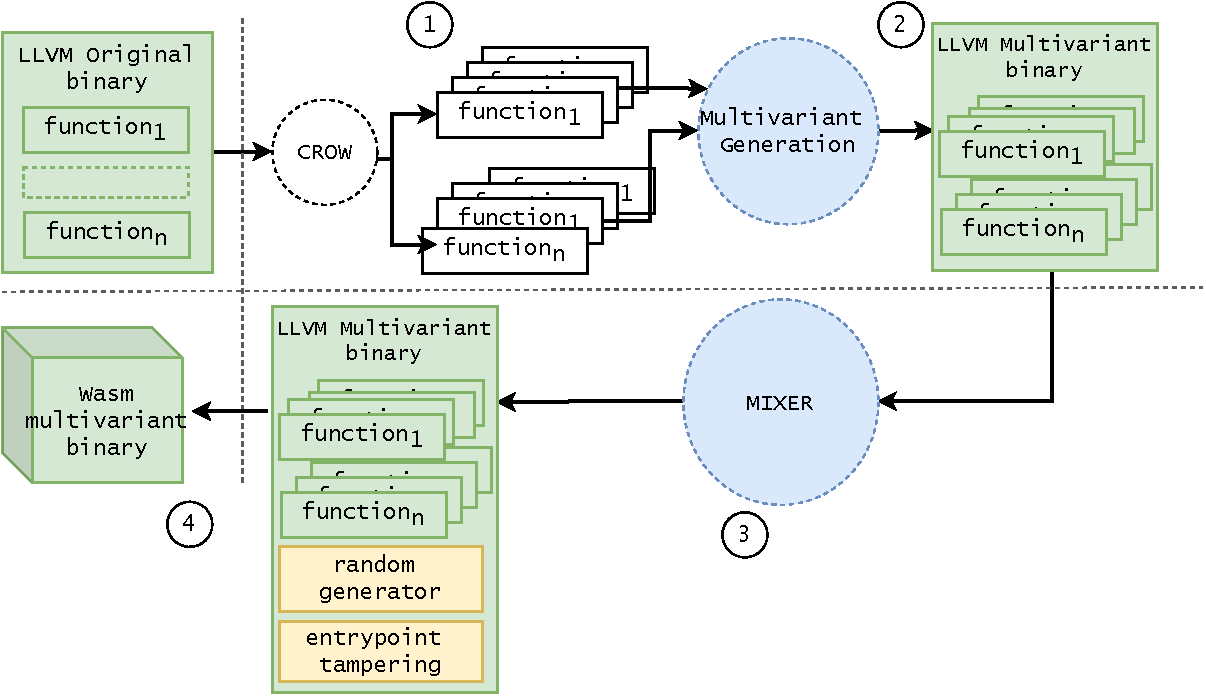
\includegraphics[height=3.2in]{diagrams/MEWE.pdf}
  \caption{Overview of \tool workflow. It takes as input an LLVM binary. It first generates a set of functionally equivalent variants for each function in the binary using CROW. Then, MEWE generates an LLVM multivariant binary composed of all the function variants. Finally, the Mixer includes the behavior in charge of selecting a variant when a function is invoked. Finally, the \tool mixer composes the LLVM multivariant binary with a random number generation library and tampers the original application entrypoint. The final process produces a \wasm multivariant binary ready to be deployed. }
  \label{workflow}
\end{figure*}


\subsection{Multivariant generation}


The key component of \tool consists in combining the variants into a single binary.
The goal is to support execution-path randomization at runtime.
The core idea is introducing one dispatcher function per original function with variants.
A dispatcher function is a synthetic function in charge of choosing a variant at random when the original function is called.
With the introduction of the dispatcher function,  \tool turns the original call graph into a multivariant call graph, defined as follows. 

\begin{definition}{Multivariant Call Graph (MCG):}\label{def:EP}
    A multivariant call graph is a call graph $\langle N, E \rangle$ where the nodes in $N$ represent all the functions in the binary and an edge $(f_1,f_2) \in E$ represents a possible invocation of $f_2$ by $f_1$  \cite{ryder1979}, where the nodes are typed. The nodes in $N$ have three possible types: a function present in the original program,  a generated function variant, or a dispatcher function.
\end{definition}


\begin{figure}
    \centering
  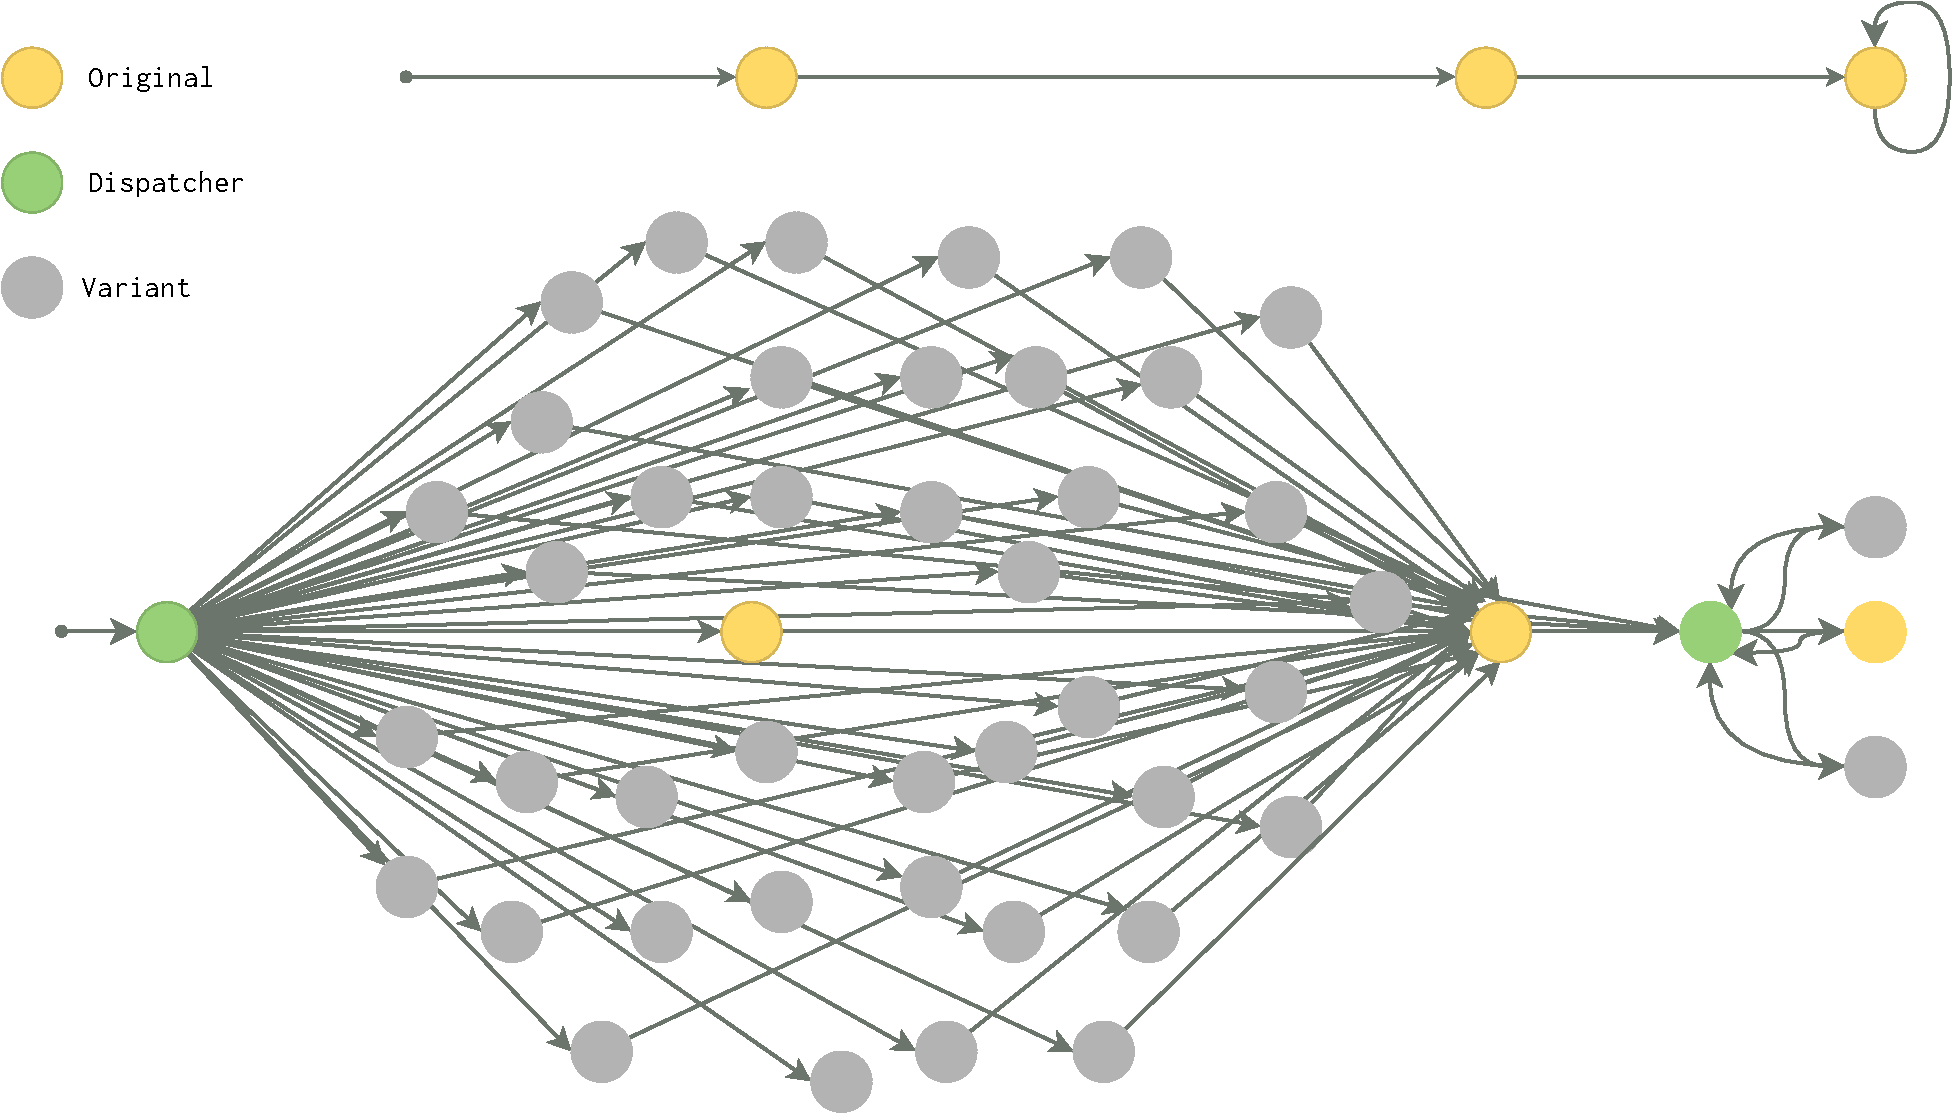
\includegraphics[width=.8\linewidth]{diagrams/CFG.pdf}
  \caption{Example of two static call graphs. At the top, the original call graph, at the bottom, the multivariant call graph, which includes nodes that represent function variants (in grey), dispatchers (in green), and original functions  (in yellow).
}
  \label{multivariant}
\end{figure}

% Instance of a multivariant module
In \autoref{multivariant}, we show the original static call graph for and original program (top of the figure), as well as the multivariant call graph generated with \tool (bottom of the figure).
The grey nodes represent function variants, the green nodes function dispatchers, and the yellow nodes are the original functions.
The directed edges represent the possible calls.
The original program includes three functions. \tool generates 43 variants for the first function, none for the second, and three for the third. 
\tool introduces two dispatcher nodes for the first and third functions. Each dispatcher is connected to the corresponding function variants to invoke one variant randomly at runtime.


% exaplanation of dispatcher
In  \autoref{listing:multivariant_template}, we illustrate the LLVM construction for the function dispatcher corresponding to the right most green node of \autoref{multivariant}.
It first calls the random generator, which returns a value used to invoke a specific function variant. 
We implement the dispatchers with a switch-case structure to avoid indirect calls that can be susceptible to speculative execution-based attacks \cite{Narayan2021Swivel}. 
The choice of a switch-case also avoids having multiple function definitions with the same signature, which could increase the attack surface in case the function signature is vulnerable \cite{johnson2021}.
This also allows \tool to inline function variants inside the dispatcher instead of defining them again.
Here we trade security over performance since dispatcher functions that perform indirect calls, instead of a switch-case,  could improve the performance of the dispatchers as indirect calls have constant time.
%It should be noted that the dispatcher function is constructed using the same signature as the original function. 


\lstset{
    language=llvm,
    %style=nccode,
    basicstyle=\footnotesize\ttfamily,
    columns=fullflexible,
    breaklines=true,
    numbers=none,
    stepnumber=1,
    float
}

\begin{code}
\scriptsize
\noindent\begin{minipage}[b]{\linewidth}
    \begin{minipage}[t]{1\linewidth}
        \begin{lstlisting}[escapeinside={(*}{*)}]
define internal i32 @foo(i32 %0) {
    entry:
      %1 = call i32 @discriminate(i32 3)
      switch i32 %1, label %end [
        i32 0, label %case_43_
        i32 1, label %case_44_
      ]
    case_43_:                 
      %2 = call i32 @foo_43_(%0)
      ret i32 %2
    case_44_:                
      %3 = <body of foo_44_ inlined>
      ret i32 %3
    end:                                             
      %4 = call i32 @foo_original(%0)
      ret i32 %4
}
        \end{lstlisting}
    \end{minipage}%
    
    \noindent\rule{\linewidth}{0.4pt}
    \captionof{lstlisting}{Dispatcher function embedded in the multivariant binary of the original function in the rightmost green node in \autoref{multivariant}.}\label{listing:multivariant_template}
\end{minipage}
\end{code}

\subsection{The Mixer}

MEWE has four specific objectives: link the LLVM multivariant binary, inject a random generator, tamper the application's entrypoint, and merge all these components into a multivariant \wasm binary.
We use the Rustc compiler\footnote{\url{https://doc.rust-lang.org/rustc/what-is-rustc.html}} to orchestrate the mixing.
For the random generator, we rely on WASI's specification \cite{WASI} for the random behavior of the dispatchers. However, its exact implementation is dependent on the platform on which the binary is deployed.
The Mixer creates a new entrypoint for the binary called \emph{entrypoint tampering}.
It wraps the dispatcher for the entrypoint variants as a new function for the final Wasm binary and is declared as the application entrypoint. 
